% Standalone ICML-style draft. Replace the preamble with the official style
% file at submission time; the body and bibliography are venue-ready LaTeX.
\documentclass[10pt,twocolumn]{article}
\usepackage[margin=0.72in,columnsep=0.24in]{geometry}
\usepackage[T1]{fontenc}
\usepackage[utf8]{inputenc}
\usepackage{lmodern,microtype}
\usepackage{amsmath,amssymb,amsthm,mathtools}
\usepackage{booktabs,graphicx,enumitem,xcolor}
\usepackage[round,authoryear]{natbib}
\usepackage[hidelinks]{hyperref}
\usepackage[nameinlink,noabbrev]{cleveref}

\setlength{\emergencystretch}{2em}
\setlist{nosep,leftmargin=*}
\newtheorem{theorem}{Theorem}
\newtheorem{lemma}[theorem]{Lemma}
\newtheorem{corollary}[theorem]{Corollary}
\newtheorem{proposition}[theorem]{Proposition}
\newcommand{\E}{\mathbb{E}}
\newcommand{\Prb}{\mathbb{P}}
\newcommand{\SNR}{\operatorname{SNR}}

\title{Critical Memory in Stateful Pricing Learners:\\
Exponential Late-Credit Gaps}
\author{Anonymous Authors}
\date{}

\begin{document}
\maketitle

\begin{abstract}
A stateful allocation rule can make a profitable price cut hard to learn
without making it unprofitable.  We study a buyer that temporarily penalizes a
seller after a cut.  The resulting MDP has two boundaries: a rational memory
threshold above which staying high is optimal and a finite-time threshold above
which fresh evidence for a profitable persistent cut is exponentially rare.
After downstream values become usable, a learner cutting with conditional
probability at most $q$ sees a fresh length-$M$ path within $T$ steps with
probability at most $Tq^M$.  A path-equivalent commitment option reduces path
proposal time to linear while preserving feasible primitive paths and optimal
value.  In a frozen numerical game, primitive Q-learning chooses the rational
action in 1/20 seeds at $M=7$, versus 19/20 with the option; paired regret falls
by 0.0643 (95\% interval $[0.0493,0.0755]$).  All seeds cover every state--action
pair, but failed learners stop revisiting deep cut states; ordered batch Bellman
sweeps recover the optimum in 20/20.  The option overcuts beyond the rational
boundary.  The result isolates a temporal credit mechanism, not live-provider
collusion.
\end{abstract}

\section{Introduction}

Independent pricing algorithms can coordinate through market feedback even
without communication.  Existing results emphasize reward signal quality,
parallel experimentation, and the scoring rule faced by each learner
\citep{hansen2021,calvano2020}.  A different friction appears when a platform
itself remembers actions.  A price cut can pay poorly today, yet become
profitable only after enough consecutive cuts erase a ranking penalty.  No
single experiment reveals the long-run return.

AI inference routing is one possible application, but current routing data do
not identify this state.  Public menus measure contemporaneous prices; owned
choices can eventually identify a current reduced-form score.  Neither shows
that the score remembers earlier prices or quality.  No paid probe randomizes a
memory rule.  We therefore use no market-share estimate as evidence for the
temporal mechanism in this paper.  The object here is the learning problem
conditional on a declared history-dependent allocation rule.

This distinction matters for both algorithmic-collusion and mechanism-design
claims.  A high learned price can arise because high pricing is an equilibrium,
because experiments are statistically coupled, or because a learner never
discovers a profitable delayed path.  These mechanisms demand different
interventions.  More exploration addresses the last mechanism only at an
exponential cost; changing the action interface can solve it but may induce
overcommitment.

Our contributions are fourfold.
\begin{enumerate}
  \item We derive an exact \emph{rational} boundary $M^*$ for persistent
  cutting under a finite-memory penalty.  It separates environments where the
  long-run low price is optimal from those where the high price is optimal.
  \item We derive a distinct \emph{learning} boundary.  After any stopping
  time $\sigma$, an adaptive policy whose cut probability is at most $q$ has
  conditional probability at most $Tq^M$ of producing a fresh length-$M$ path
  within $T$ steps.  Combining this bound with ordinary reward estimation
  separates late temporal credit from reward SNR.
  \item We show that a length-$(M+1)$ commitment option preserves the optimal
  value and feasible primitive paths while replacing exponential path-proposal
  time by a linear term.  This is an interface result, not a change in provider
  payoffs.
  \item We test the mechanism in a frozen, prespecified finite MDP.  The option
  closes the local gap at intermediate memory and becomes harmful beyond the
  rational boundary.  A frozen trace replay separates early discovery from late
  credit starvation.  State observability, cross-market severity, and a
  conventional multi-step return each fail prespecified tests.
\end{enumerate}

\section{Stateful pricing game and economic boundary}

A seller repeatedly chooses a high quote $H$ or low quote $L$.  The buyer's
declared allocation rule carries a binary penalty state.  A low quote remains
penalized until the previous $M$ quotes are also low; after that run, the
penalty clears.  The state can represent a prominence rule, a reserve-ranking
flag, or any other disclosed history-dependent procurement policy.  We do not
assume that a particular live router implements it.

Let $u_H$ be seller profit at $H$, $u_{\theta L}$ penalized profit at $L$, and
$u_L$ unpenalized profit at $L$.  These quantities may be generated by any
demand or allocation system.  The theory requires only the economically
interesting
ordering is
\begin{equation}
  u_L>u_H>u_{\theta L}.
  \label{eq:ordering}
\end{equation}
ordering: cutting loses while the flag is active but wins after it clears.

\begin{theorem}[Rational memory boundary]
From an all-high history, an infinite-horizon optimal policy either stays high
forever or cuts immediately and stays low.  For discount $\gamma\in(0,1)$,
cutting is strictly optimal iff
\begin{equation}
 \gamma^M>
 \frac{u_H-u_{\theta L}}{u_L-u_{\theta L}}.
 \label{eq:rational-boundary}
\end{equation}
The continuous boundary is
$M^*=\log[(u_H-u_{\theta L})/(u_L-u_{\theta L})]/\log\gamma$.
\label{thm:rational}
\end{theorem}

In the frozen numerical profile,
$(u_H,u_{\theta L},u_L)=(0.1067535,0.0351280,0.1501829)$ and
$\gamma=0.95$, giving $M^*=9.2402$.  Exact dynamic programming cuts for
integer $M\le9$ and stays high for $M\ge10$.  This boundary is derived before
examining learning outcomes.

\section{Critical memory for finite-time learning}

Let $A_t\in\{H,L\}$.  Fix any stopping time $\sigma$ representing a stage
at which downstream reward or value information has become usable, and define
$\tau_M(\sigma)$ as the first $t\ge\sigma+M$ for which the $M$ actions after
$\sigma$ ending at $t$ are all low.  This definition is intentionally
conditional: an early visit can reveal the terminal reward without supplying a
later one-step learner enough fresh support to propagate that value upstream.
We allow full history dependence and require only
\begin{equation}
 \Prb(A_t=L\mid\mathcal F_{t-1},\,t>\sigma,\,
 \tau_M(\sigma)\ge t)\le q.
 \label{eq:qcap}
\end{equation}

\begin{theorem}[Exponential fresh-path barrier]
Under \cref{eq:qcap}, for every horizon $T$ and almost every realized
$\mathcal F_\sigma$,
\begin{equation}
 \Prb(\tau_M(\sigma)\le\sigma+T\mid\mathcal F_\sigma)
 \le (T-M+1)_+q^M\le Tq^M.
 \label{eq:discovery-bound}
\end{equation}
Consequently, attaining conditional fresh-path probability at least
$1-\delta$ requires
\begin{equation}
 T\ge (1-\delta)q^{-M}.
 \label{eq:horizon-lower}
\end{equation}
If post-$\sigma$ actions are iid Bernoulli$(q)$, the exact expected additional
time is
\begin{equation}
 \E[\tau_M(\sigma)-\sigma\mid\mathcal F_\sigma]
 =\frac{1-q^M}{(1-q)q^M}.
 \label{eq:exact-wait}
\end{equation}
\label{thm:critical}
\end{theorem}

Define the finite-horizon critical memory
\begin{equation}
 M_c(T,q,\delta)=
 \left\lfloor\frac{\log[T/(1-\delta)]}{\log(1/q)}\right\rfloor.
 \label{eq:critical-memory}
\end{equation}
For $M\ge M_c+1$, the target fresh-path probability is ruled out after any
chosen readiness time $\sigma$.  Thus memory is a computational control
parameter for learners that need fresh downstream support: increasing $T$ by a
factor of ten buys only $1/\log_{10}(1/q)$ additional memory periods.

This clarifies the relationship to signal-to-noise results.  Suppose
reward differences are sub-Gaussian with gap $\Delta$ and proxy variance
$\sigma^2$.  Then $O(\SNR^{-1}\log(1/\delta))$ samples, where
$\SNR=\Delta^2/\sigma^2$, suffice to identify the better downstream action.
If upstream credit requires a fresh path after that readiness stage,
\cref{eq:horizon-lower} still applies.

\begin{corollary}[Temporal--statistical crossover]
For a fixed-confidence ordered-credit learner, total difficulty contains a
fresh-support term $q^{-M}$ and a statistical term
$\SNR^{-1}\log(1/\delta)$.  Temporal discovery dominates once
\begin{equation}
 q^{-M}\gg \SNR^{-1}\log(1/\delta).
\end{equation}
Higher reward SNR cannot remove this conditional gap; it moves the readiness
time $\sigma$ but does not change post-$\sigma$ path probability.
\label{cor:snr}
\end{corollary}

The result complements Hansen--Misra--Pai: independent experiments may couple
through the final pricing score even with no explicit memory
\citep{hansen2021}.  Our theorem does not contradict asymptotic learnability.
It supplies a finite-time rate: once market memory requires a run rather than
an isolated experiment, the time needed to re-expose the relevant score after
downstream learning can be exponential in $M$.  This conditional statement is
not, by itself, an explanation of the Q-learning result; the trace audit below
tests whether late support is actually absent.

\section{A path-equivalent intervention}

Augment the primitive MDP with a \texttt{commit-low} option that executes
$M+1$ existing low actions.  Both primitive actions remain available.

\begin{theorem}[Value preservation and linear discovery]
The augmented semi-Markov MDP has exactly the same optimal value as the
primitive MDP at every state.  It creates no new primitive price path.  If the
option is selected independently with probability $q_o$ at each decision
epoch while non-option decisions consume one transition, its completion time
has expectation
\begin{equation}
  M+q_o^{-1}.
  \label{eq:option-wait}
\end{equation}
\label{thm:option}
\end{theorem}

The option changes representation, not incentives.  Any augmented policy can
be unrolled into the same sequence of primitive actions and discounted
rewards.  But the probability of proposing the full low path is now $q_o$
rather than $q^M$.  This is the exponential temporal-abstraction gap shown in
\cref{fig:critical}A.

\begin{figure*}[t]
 \centering
 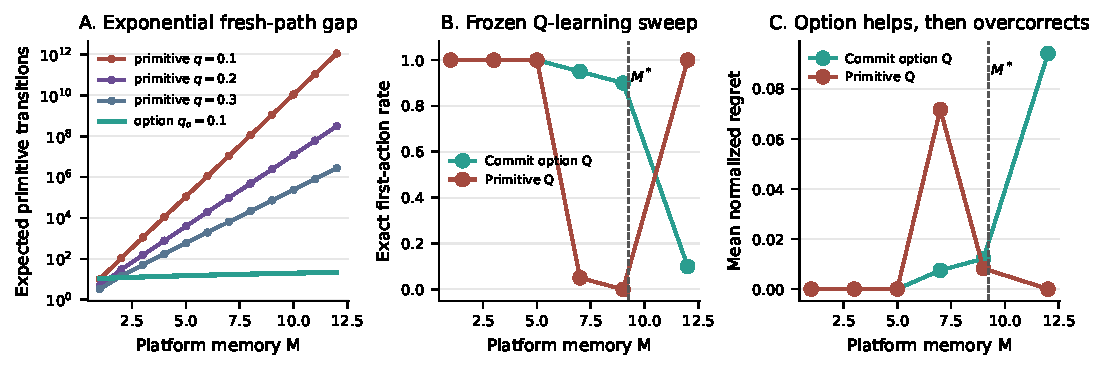
\includegraphics[width=0.98\textwidth]{critical-memory.pdf}
 \caption{Theory and frozen experiment.  A: after any readiness checkpoint,
 iid primitive exploration takes exponential additional time to produce a
 fresh length-$M$ cut path; a commitment option is linear in $M$.  B: exact
 first-action agreement over 20 seeds.  C: mean
 normalized regret.  The dashed rational boundary $M^*=9.2402$ is computed
 from payoffs, not fitted to learner outcomes.}
 \label{fig:critical}
\end{figure*}

\section{Experimental design}

The experiment is a controlled finite-MDP mechanism test, not a reduced-form
test on observed seller prices.  Its high and low quotes, payoffs, and penalty
are frozen before simulation and chosen to satisfy \cref{eq:ordering}; they are
not structural estimates from a live marketplace.  Exact value iteration supplies the target
action.  Tabular Q-learning uses 300,000 primitive transitions, discount
$0.95$, and 20 prespecified seeds.  The option learner receives the same
primitive transition budget; an option consumes its full duration.  A
10,000-transition frozen-policy evaluation reports first-action agreement and
normalized regret.  Paired seed bootstrap intervals describe simulation
variation only.

We use a falsification ladder rather than interpreting one favorable run.
E-SIM5 gives the primitive learner the complete Markov history.  E-SIM6 adds
only the path-equivalent option and sweeps
$M\in\{1,3,5,7,9,12\}$.  E-SIM7 transports the intervention to four frozen
price books.  E-SIM8 varies learning rate and exploration decay in a $3\times3$
 grid.  E-SIM9 replaces one-step Q with an eight-step TD target while retaining
 the primitive action set.  All gates, seeds, and result hashes were frozen
 before interpretation.

After freezing E-SIM6, we added a descriptive trace audit rather than modifying
its confirmatory gate.  It replays the exact 20 primitive seeds, asserts every
terminal Q-table against the frozen artifact to tolerance $10^{-12}$, records
trailing-low-state visits after steps 100,000 and 200,000, and reconstructs the
deterministic empirical transition table from visited pairs.  Batch Bellman
sweeps then test whether coverage is sufficient when update order is repaired.
The checkpoints are diagnostics, not preregistered readiness estimates.

\paragraph{External-market non-entry statement.}
The repository also contains public-menu shadow-share accounting and a
prospective owned-choice score estimator.  Neither artifact enters the payoffs,
memory length, transition law, or result selection in this paper.  A
contemporaneous score wedge cannot identify $M$; price persistence cannot show
that the buyer stores price history; and no existing probe randomizes memory.
Connecting this theorem to inference routing is therefore a future transport
test, not an empirical contribution of this draft.

\section{Results}

\paragraph{Critical memory is visible in learning.}
At $M\in\{1,3,5\}$, primitive and option learners agree with exact control in
20/20 seeds.  At $M=7$, where exact optimization still cuts, primitive Q agrees
in 1/20 seeds while option Q agrees in 19/20; 18/20 option seeds also satisfy
the joint low-regret gate.  At $M=9$, the comparison is 0/20 versus 18/20.
The transition is therefore near, but below, the independently derived
rational boundary.

At $M=7$, mean normalized regret is $0.07175$ for primitive Q and $0.00750$
for option Q.  The paired difference is $-0.06425$ with 95\% seed-bootstrap
interval $[-0.07553,-0.04930]$.  The sign remains negative in every one of
nine learning-rate/exploration-decay cells; the strict composite severity gate
passes in seven.

\paragraph{Early discovery is not the explanation.}
The trace audit reproduces all 20 frozen Q-tables exactly.  Every primitive
learner reaches the all-low state early: first-hit times range from step 7 to
901.  Every seed also observes every one of the 256 state--action pairs at
least nine times.  Nevertheless, 19 finish with the wrong high initial action.
Among those failures, none visits a state with five or more trailing low
actions after step 100,000, and none returns to the all-low state.  Thus neither
first discovery nor aggregate support is the explanation.  Ordered batch
Bellman sweeps on each seed's same observed deterministic transitions recover
the exact initial cut in 20/20 seeds.  The observed mechanism is therefore
\emph{late credit starvation}: the data needed to solve the model were
collected while exploration was broad, but online one-step updates did not
revisit deep states after downstream values separated.  This diagnostic
motivates the stopping-time formulation of \cref{thm:critical}; it does not
estimate a unique readiness time.

\paragraph{The intervention is nonmonotone.}
At $M=12$, exact optimization stays high.  Primitive Q is correct in 20/20
seeds, whereas option Q is correct in only 2/20 and adds $0.0942$ normalized
regret.  An interface that solves delayed credit can therefore reduce
welfare when it creates commitment salience on the wrong side of the economic
boundary.  Mechanism evaluation must combine \cref{thm:rational} with
\cref{thm:critical}; the learning boundary alone is not a design objective.

\paragraph{The falsifications narrow the mechanism.}
Complete state observability does not repair primitive learning: it remains
high in 19/20 seeds at $M=7$.  The severe-trap transport gate fails in two of
four external price books, although all four option-effect signs align with
their rational boundary.  Finally, an ordinary eight-step TD target succeeds
in 0/20 seeds and has regret difference $+0.0038$ relative to one-step Q,
interval $[0,0.0113]$.  The supported result is option-specific temporal
abstraction in the controlled MDP, not a claim that any longer return solves
delayed credit.

\section{Implications for stateful platform design}

The two boundaries separate three regimes.
\begin{enumerate}
 \item If $M>M^*$, a persistent cut destroys provider value.  High pricing is
 rational; exploration policy is secondary.
 \item If $M\le M^*$ but $M>M_c(T,q,\delta)$, cutting is rational but is
 unlikely to receive a fresh length-$M$ support path within the late-learning
 horizon.  A platform can sustain high learned prices without communication or
 supra-rational reward coupling.
 \item If $M\le\min\{M^*,M_c\}$, ordinary exploration can expose the low path;
 ordinary reward noise and unmodeled cross-agent feedback again become first-order.
\end{enumerate}

This yields a design warning.  Platform memory can look anti-gaming because it
disciplines short-lived cuts, yet the same rule can suppress efficient
persistent cuts by altering learnability.  Conversely, exposing a commitment
action can restore price competition below $M^*$ but cause excessive cutting
above it.  A safer platform would expose the state and a cancellable multi-period
quote schedule only when a deviation audit predicts that persistent cutting
raises provider value and buyer surplus.  The theorem supplies a testable
screen, not a universally optimal policy.

\paragraph{Illustrative inference-routing application.}
The target score must also match the economic objective.  A user-cost router
scores payment, latency, and failure; a welfare router substitutes resource cost
for payment and values delivered quality; a revenue router may favor high spend
under ad-valorem fees; and a quality-priority router maximizes verified fidelity
subject to budget.  These objectives generate different payoff triples and
hence different $M^*$.  The commitment option should be evaluated on a Pareto
frontier over user cost, welfare bounds, router revenue, quality, completion,
and provider exploitability rather than on price alone.

Provider technology shifts the same boundary.  An owned or reserved-capacity
provider pays high fixed cost but may rationally cut to maintain utilization; a
spot-dependent provider has less sunk exposure but state-dependent scarcity
cost; an anchor adopter may not update displayed price at all.  A router that
hides score memory can therefore trap low-short-run-cost providers while doing
little to passive anchors.  This is a theoretical comparative static, not an
interpretation of the current provider panel.  Practical implementation should
expose the score
state, offer cancellable multi-period quote commitments, use
execution-contingent capacity rather than fundraising or provider identity as a
proxy, and charge fees separately from selected spend.

\section{Related work}

Algorithmic-pricing research establishes that independent learners may
support high prices and that results depend sharply on algorithms and timing
\citep{calvano2020,asker2022,brownmackay2023}.  Hansen--Misra--Pai show how
independent bandit experiments become strategically coupled through the
aggregate price used to score arms \citep{hansen2021}.  Johnson--Rhodes--
Wildenbeest study platform steering when sellers use pricing algorithms
\citep{johnson2023}.  Our contribution is orthogonal: a platform's own-history
rule creates a finite-time fresh-support barrier even when reward differences
are otherwise easy to estimate.

Options and semi-Markov value preservation are classical
\citep{sutton1999}; delayed reward and sequence compression have recently been
studied directly \citep{han2022,ramesh2024}.  We add an economic source of the
delay, an explicit critical-memory rate, a rational boundary with the opposite
comparative-static force, and controlled evidence that the representation
intervention helps only between those boundaries.

\section{Limitations and claim boundary}

The finite-time theorem assumes a post-stopping-time cut-probability cap and
applies only to learners that require fresh downstream support.  It does not
characterize algorithms that plan over a known model, retain replay sufficient
for exact offline backups, or deliberately schedule low runs.  The diagnostic
checkpoint is post hoc and does not identify when a Q-value becomes usable.
The controlled experiment fixes rivals, uses two prices, and studies tabular Q.
Twenty seeds identify Monte Carlo variability, not uncertainty in live-market
parameters.  Cross-profile severe-trap transport fails, and no paid probe
randomizes a memory rule.  We therefore claim a theorem, a controlled mechanism,
and a reproducible numerical counterfactual---not observed market share,
provider intent, tacit collusion, communication, or live-router causality.

\section{Conclusion}

Platform memory creates two distinct thresholds.  The rational threshold says
whether persistent cutting is valuable; the finite-time threshold says whether
a bounded ordered-credit learner can obtain fresh support after its downstream
values become usable.  Between them, high learned prices can persist despite a
profitable low-price path, with late path time exponential in memory and only
logarithmic improvement from longer training.  Complete state--action coverage
is insufficient for the online learner, while ordered batch backups on those
same transitions recover the optimum.  A path-equivalent option also collapses
that gap but overcorrects when cutting is no longer rational.  Learning-aware
marketplace design must therefore optimize
both incentives and representations, then audit deviations on either side of
the boundary.

\appendix
\section{Proofs}

\begin{proof}[Proof of \cref{thm:rational}]
Once the history is all-low, $L$ strictly dominates $H$ by
\cref{eq:ordering}; choosing $H$ also restarts the penalty.  Before that state,
any policy that eventually cuts is weakly improved to $k$ high actions followed
by low forever.  Its value is
\begin{align*}
 V_k&=\frac{u_H(1-\gamma^k)}{1-\gamma}+\gamma^kV_{\rm cut},\\
 V_{\rm cut}&=\frac{(1-\gamma^M)u_{\theta L}+\gamma^Mu_L}{1-\gamma}.
\end{align*}
Because
$V_k-u_H/(1-\gamma)=\gamma^k[V_{\rm cut}-u_H/(1-\gamma)]$, either $k=0$
or never cutting is optimal.  Comparing these alternatives yields
\cref{eq:rational-boundary}.
\end{proof}

\begin{proof}[Proof of \cref{thm:critical}]
Condition on $\mathcal F_\sigma$.  For each candidate ending time
$t>\sigma$, iterated conditioning and \cref{eq:qcap} bound the probability
of the required post-$\sigma$ all-low length-$M$ window by $q^M$.  A union
bound over $(T-M+1)_+$ windows proves
\cref{eq:discovery-bound}; inversion of its looser $Tq^M$ form gives
\cref{eq:horizon-lower}.  Under iid Bernoulli exploration, let $E_k$ be the
expected remaining time after a current run of $k$ lows.  The recursions
$E_M=0$ and $E_k=1+qE_{k+1}+(1-q)E_0$ solve to
$E_0=(1-q^M)/[(1-q)q^M]$.
\end{proof}

\begin{proof}[Proof of \cref{thm:option}]
The augmented action set contains every primitive action, so its optimal value
is weakly larger.  Replace each option in any augmented policy by its defining
$M+1$ primitive low actions.  The unrolled policy produces identical states,
durations, and discounted rewards, so its value is identical and the augmented
optimum cannot be larger.  Before the first option, the number of one-step
decisions is geometric with mean $(1-q_o)/q_o$; adding the final $M+1$
transitions gives $M+q_o^{-1}$.
\end{proof}

\section{Reproducibility}

The theory functions and unit tests are in
\texttt{src/orcap/market\_env/critical\_memory.py} and
\texttt{tests/market\_env/test\_critical\_memory.py}.  The figure is generated
directly from the frozen E-SIM6 parquet.  Clean bundles are E-SIM5
\texttt{3e5a55405e}, E-SIM6 \texttt{93265b9b03}, E-SIM7
\texttt{bd74ab2eb7}, E-SIM8 \texttt{4d84b9b3a2}, and E-SIM9
\texttt{179eca0f9d}.  Manifests pin source commits, seeds, result hashes, and
input-artifact hashes.  Exact Bellman residuals, path equivalence, paper
numbers, and the new finite-time identities are enforced by tests.
The post-hoc trace artifact
\texttt{credit-propagation-diagnostic.json} is generated by the adjacent
replay script.  It is admitted only after all 20 Q-tables match the frozen
E-SIM6 artifact; separate tests reconcile seed-level actions, early hits, and
late depth counts.
The separate price--score evidence ledger is not an input to this paper's
payoffs, memory length, transition law, or confirmatory gates.  This exclusion
is intentional and is checked in the manuscript evidence audit.

\bibliographystyle{plainnat}
\begingroup
\scriptsize
\setlength{\bibsep}{0pt plus 0.3ex}
\bibliography{references}
\endgroup

\end{document}
